\subsection{Czarne dziury Schwarzschilda}

Czarne dziury fascynują i przerażają. Są to obiekty rodem z science fiction - punkt o zerowej objętości i nieskończonej gęstości otoczony tajemniczym horyzontem zdarzeń. Nic dziwnego, że sam Einstein, jak i wielu naukowców, nie mogli uwierzyć w ich istnienie.

Czarne dziury powstają w wybuchu supernowej, kiedy gwieździe skończy się paliwo, a reakcje termojądrowe zatrzymają się, grawitacja zgniata masę do jednego malutkiego punktu - osobliwości. Jego masa jest tak wielka, że zakrzywia czasoprzestrzeń i spowalnia czas, a linia po której przekroczeniu nic, nawet światło, nie jest w stanie uciec, nazywamy horyzontem zdarzeń. 

Czarne dziury były inspiracją dla wielu autorów gatunku science fiction - w filmie \emph{Interstellar} pojawia się Gargantua - obiekt o masie 100 milionów Słońc. Gdy podróżnicy docierają na planetę orbitującą wokół czarnej dziury mówią, iż czas płynie tu wolniej. Zjawisko możemy potwierdzić patrząc na wykres, pokazujący stosunek czasu płynącego normalnie, do czasu w zakrzywionej czasoprzestrzeni.

\renewcommand{\figurename}{Wykres}
\begin{figure}[h]
  \centering
  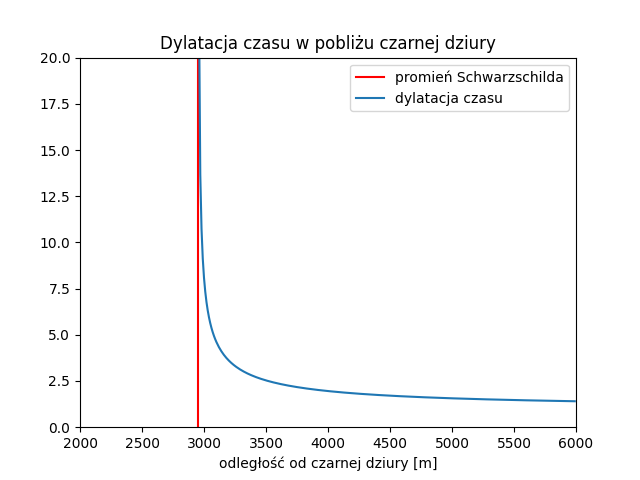
\includegraphics[width=0.7\textwidth]{ilustracje/Time_near_black_hole.png}
  \caption{Stosunek upływu czasu własnego do upływu czasu obserwowanego w punkcie nieskończenie odległym od czarnej dziury w zależności od położenia $r$.}
  %supplement: [Wykres]
%) <time_dilation>
\end{figure}

W 2019 roku otrzymaliśmy pierwsze zdjęcie czarnej dziury, natomiast w maju 2022 roku otrzymaliśmy zdjęcie Saggitariusa A. - jest to supermasywny obiekt w centrum naszej galaktyki \ref{zakazany donut}.

\renewcommand{\figurename}{Zdjęcie}
\begin{figure}[h]
  \centering
  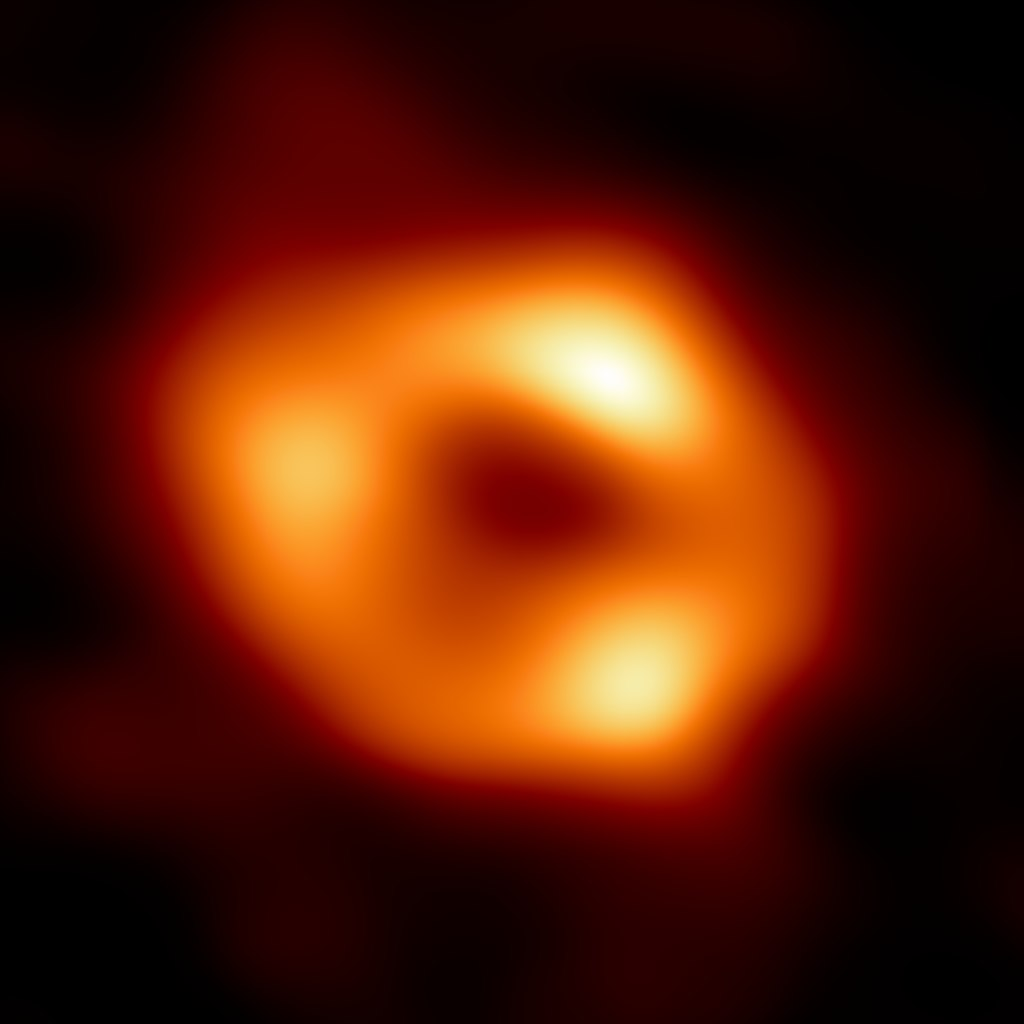
\includegraphics[width=0.7\textwidth]{ilustracje/zakazany_donut.jpg}
  \caption{Zdjęcie czarnej dziury w centrum Mlecznej Drogi uzyskane przez \cite{mleczna_droga}}\label{zakazany donut}
%  supplement: [Figura]
%) <time_dilation>
\end{figure}

Z matematycznego punktu widzenia, czarna dziura jest rozmaitością różniczkowalną z tensorem metrycznym, który opisuje jak zakrzywiona jest przestrzeń wokół niej. Aby więc dokładnie zrozumieć jak zachowują się cząsteczki w jej pobliżu, należy zrozumieć czym są rozmaitości.% i jak wygląda ich geometria.
